\documentclass[a4paper,oneside,11pt]{book}
\usepackage{NWUStyle}
\usepackage{titlesec} % For redefining chapter title format
\usepackage{tocloft} % For customizing table of contents
\usepackage{titlesec}
\usepackage{graphicx}
\usepackage{enumitem}
\usepackage{pdfpages}
\usepackage{float} 
% Redefine chapter and section spacing
\titlespacing{\chapter}{0pt}{-50pt}{5pt} % Adjust the spacing as needed
\titlespacing{\section}{0pt}{10pt}{5pt} % Adjust the spacing as needed
\titlespacing{\subsection}{0pt}{10pt}{5pt} % Adjust the spacing for subsections
\titlespacing{\subsubsection}{0pt}{10pt}{5pt} % Adjust the spacing for subsubsections

% Ensure subsubsections are included in the table of contents
\setcounter{tocdepth}{3}
\setcounter{secnumdepth}{3}

\titleformat{\chapter}[display]
{\normalfont\huge\bfseries}{}{0pt}{\Huge}

\begin{document}
\Title{Documentation / Report on the Deep Learning Model for Fruit Quality Classification}
\Initials{B.}
\FirstName{Bernard}
\Surname{Swanepoel}
\StudentNumber{39909476}
\Supervisor{Prof. Absalom El-Shamir Ezugwu}
\MakeTitle 

\pagenumbering{roman} 
\tableofcontents

% Ensure the list of figures is on a new page
\newpage
\setcounter{page}{2}
\listoffigures

\cleardoublepage 
\pagenumbering{arabic} 

\chapter{Introduction}
Farmers produce a variety of fruits each year, which are sold globally. As fruits age and rot, they can pose health risks \citep{sudhakara2022statistical}. An AI model can be developed to detect these signs on fruit skins, reducing the risk of illness from spoiled fruit.
\section{Aims and Objectives}
\subsection{Aims}
The primary aim of this research is to develop a robust machine learning model for assessing fruit quality using image data. The model will use deep learning techniques, specifically Convolutional Neural Networks (CNNs), to classify fruit quality based on different attributes visible in images. This research aims to enhance the accuracy and efficiency of fruit quality assessment, assisting agricultural practices and consumer markets.
\subsection{Objectives}
\begin{itemize}
    \item To preprocess and prepare fruit image data for training a CNN model.
    \item To design and implement a CNN architecture suitable for fruit quality classification.
    \item To evaluate and optimize the model's performance using numerous hyperparameters and preprocessing techniques.
    \item To integrate the trained model into an application for real-time fruit quality assessment using React Native and PyTorch.
\end{itemize}
\section{Problem Statement}
Accurate fruit quality assessment is important for maintaining high agricultural standards. Traditional inspection methods are labor-intensive and error-prone, risking food safety. This research aims to automate fruit quality assessment using machine learning to enhance accuracy and reduce manual effort.
\section{Research Question}
How can Convolutional Neural Networks classify fruit quality from images, and how do preprocessing techniques, model architectures, and hyperparameters affect performance?
\pagestyle{plain}
\chapter{Short Literature Review}
% \section{Literature review topics}
% \textbf{The following topics will be covered:}
% \begin{itemize}
%     \item Convolutional Neural Network (CNN)
%     \item Explainable Artificial Intelligence (XAI)
%     \item Model benchmarking
% \end{itemize}
% \section{Main Literature review}
\section{Convolutional Neural Network (CNN)}
Agriculture plays a crucial role in the economy, with fruit production being a key sector due to high consumer demand \citep{naranjo2020review}. To meet this demand, innovative technologies like artificial intelligence are becoming essential \citep{naranjo2020review}. Deep Learning (DL), particularly Convolutional Neural Networks (CNNs), has proven effective in image-based tasks \citep{naranjo2020review}. This review highlights the growing application of CNNs in fruit image processing, including classification, quality control, and detection \citep{naranjo2020review}. The use of CNNs for fruit recognition has surged in recent years, achieving impressive results through new models and transfer learning \citep{naranjo2020review}. The article also covers CNN fundamentals, tools, and practical examples for fruit sorting and quality control \citep{naranjo2020review}.
\section{Explainable Artificial Intelligence (XAI)}
Fruit research has advanced significantly with the help of machine learning, offering actionable insights for agricultural practitioners \citep{sahidullah2023date}. To automatically assess the edibility of date fruits, various types were analyzed using explainable artificial intelligence (XAI) combined with machine learning techniques \citep{sahidullah2023date}. Achieving 90-92\% accuracy across seven methods, including boosting, bagging, SVM, KNN, and MLPs, the integration of XAI with Local Interpretable Model-Agnostic Explanations (LIME) provided valuable insights \citep{sahidullah2023date}. These findings can help domain experts enhance fruit quality, particularly for date fruits, contributing to advancements in this rapidly evolving field \citep{sahidullah2023date}.
\section{Model benchmarking}
Harvesting, a routine crop production task, is ideal for automation. Tomatoes, a high-value crop, face challenges in robotic harvesting \citep{moreira2022benchmark}. Accurate fruit detection is key to automation. Deep Learning (DL) methods like SSD and YOLO provide robust tomato detection \citep{moreira2022benchmark}. This study compares DL models (SSD MobileNet v2 and YOLOv4) with a histogram-based HSV color space model for classification. YOLOv4 excelled in detection (F1-Score: 85.81\%) and classification (Macro F1-Score: 74.16\%), while the HSV model outperformed SSD MobileNet v2 with a Balanced Accuracy of 68.10\% \citep{moreira2022benchmark}.
\chapter{Dataset}
\section{Dataset Details}
The dataset comprises images of fruits categorized into three conditions: fresh, mild, and rotten. The fruits included are bananas, cucumbers, grapes, kaki, papayas, peaches, pears, peppers, strawberries, watermelons, and tomatoes. This dataset, available on Kaggle, is used to train the Convolutional Neural Network (CNN) to identify these fruits and classify them into the specified categories of fresh, mild, or rotten. There are two main datasets: the training dataset and the test dataset. The training dataset is used to train the model, while the test dataset is used to evaluate its performance.
\begin{figure}[H]
    \centering
    \makebox[\textwidth][c]{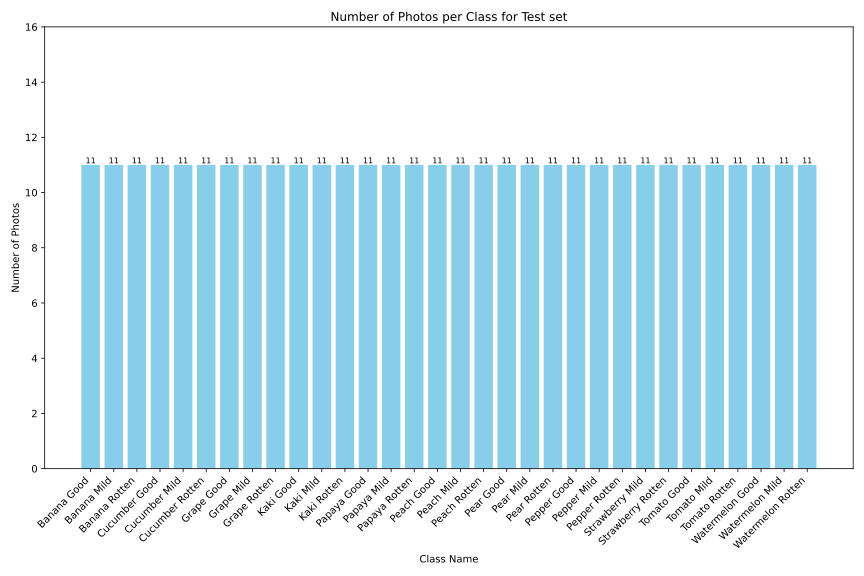
\includegraphics[width=1.2\textwidth, height=1.2\textheight, keepaspectratio]{img/Distribution_Test_Dataset.png}}
    \caption{Distribution of the test dataset.}
\end{figure}
\begin{figure}[H]
    \centering
    \makebox[\textwidth][c]{\includegraphics[width=1.2\textwidth, height=1.2\textheight, keepaspectratio]{img/Distribution_Train_Dataset.png}}
    \caption{Distribution of the train dataset.}
\end{figure}
\section{Preprocessing}
\subsection{Data Transformation}
Images are resized to 224x224 pixels, which standardizes their dimensions and ensures compatibility with the input size expected by the model, such as VGG16, which is trained on images of this size. For training data, a random horizontal flip is applied as a data augmentation technique. This introduces variability in the orientation of the images, helping the model to generalize better by learning to recognize objects regardless of their horizontal positioning. After resizing and augmentation, the images are converted to tensors. This conversion is necessary because deep learning frameworks, such as PyTorch, require input data in tensor format for efficient computation. Finally, the images are normalized using specific mean and standard deviation values ([0.485, 0.456, 0.409] for the mean and [0.229, 0.224, 0.225] for the standard deviation). Normalization adjusts the pixel values to a standard scale, with a mean of 0 and a standard deviation of 1, based on the ImageNet dataset statistics. This step is important for stabilizing the training process and improving the model's convergence by ensuring that the input data has consistent statistical properties.
\subsection{Normalization}
The mean and standard deviation values used for normalization are [0.485, 0.456, 0.406] and [0.229, 0.224, 0.225], respectively. These values correspond to the average and variability of pixel intensities in the ImageNet dataset, which is a large-scale dataset commonly used for training and evaluating image classification models. Normalizing images using these specific mean and standard deviation values helps to standardize the input data. By subtracting the mean and dividing by the standard deviation, each color channel (Red, Green, Blue) of the images is scaled to have a mean of 0 and a standard deviation of 1. This process adjusts the pixel values to fit within a consistent range, which enhances the stability of the training process and allows the model to learn more effectively. Using these normalization parameters is particularly beneficial when transferring learning from models pre-trained on ImageNet, as it ensures that the input data is processed in a way that aligns with the conditions under which the model was originally trained.
\pagestyle{plain}
\section{Matplotlib figure containing some of the images in the dataset}
\begin{figure}[H]
    \centering
    \makebox[\textwidth][c]{\includegraphics[width=1.2\textwidth, height=1.2\textheight, keepaspectratio]{img/fruitssss.png}}
    \caption{Some of the fruits in the dataset.}
\end{figure}
\chapter{Model Details}
\section{Technologies used in the model}
\begin{itemize}
    \item Google Colab: Used as the development environment to write and execute Python code. It provides access to GPU resources, which speeds up the training of your deep learning model.
    \item PyTorch: Utilized as the AI framework for developing and training the neural network model. PyTorch was used to define the neural network architecture, perform forward and backward passes, and manage the optimization process.
    \item Torchvision: Used for handling image data and transformations. It was used to load and preprocess the dataset (resizing, normalization) and to create data loaders for efficient batch processing during training and evaluation.
    \item NumPy: Used for numerical operations and data manipulation, particularly for arrays and performing calculations to model metrics and evaluations.
    \item Matplotlib: Utilized for visualizing training progress and evaluation results. It was used to plot loss curves, ROC curves, and confusion matrices to assess model performance visually.
    \item Scikit-learn: Applied for computing performance metrics such as accuracy, precision, recall, F1 score, and ROC AUC. These metrics are crucial for evaluating the model's performance on the test dataset.
    \item Seaborn: Used for creating enhanced visualizations, such as heatmaps of confusion matrices, to provide more insightful and aesthetically pleasing representations of model evaluation results.
    \item Google Drive: Used for storing and accessing datasets and model files.
\end{itemize}
\section{Hyperparameters} 
\begin{figure}[H]
    \centering
    \makebox[\textwidth][c]{\includegraphics[width=0.9\textwidth, height=0.9\textheight, keepaspectratio]{img/hyperparamets.png}}
    \caption{Hyperparameters of the model.}
\end{figure}
\subsection{Details of hyperparameters}
\begin{itemize}
    \item Trained for 150 epoch with a patience value of 10.
    The patience value is there to stop the model from overtraining when it can’t improve the model’s loss for 10 consistent epochs.
    \item Optimizer:  Creates an Adamaoptimizer with a learning rate of 0.001 to update the parameters of the model net during training.
    \item Cross-Entropy Loss: Defines the loss function for training, specifically Cross-Entropy Loss, which is commonly used for classification tasks. It measures the difference between the predicted class probabilities and the actual class labels.
    \item Scheduler:  Reduces the learning rate of the optimizer when a monitored metric (e.g., loss) has stopped improving. patience=10 means the learning rate will be reduced after 10 epochs of no improvement, and factor=0.1 specifies that the learning rate will be multiplied by 0.1 when reduced.
\end{itemize}
\section{Model Architecture: Convolutional Neural Network (CNN)}
\begin{figure}[H]
    \centering
    \makebox[\textwidth][c]{\includegraphics[width=1\textwidth, height=1.2\textheight, keepaspectratio]{img/NNArchitecture.png}}
    \caption{Architecture of the model.}
\end{figure}
\subsection{Detail of architecture}
\begin{itemize}
    \item Conv2D: A filter or kernel "slides" across the 2D input data, carrying out elementwise multiplication.
    \item BatchNorm2d: The number of dimensions or channels that are produced by the previous layer and enter the batch normalization layer.
    \item Dropout: Data or noise intentionally excluded from a neural network to enhance processing efficiency and reduce time to results.
    \item Linear / fully connected:  Applies a linear transformation to the incoming data.
    \item ReLU: Activation function.
    \item Def forward:  Defines how the input data passes through the network's layers to produce the output.
\end{itemize}
\section{Reasons for using ReLU function}
\begin{itemize}
    \item ReLU is efficient in terms of computation because it only requires thresholding the input \citep{choubey2023activation}.
    \item ReLU helps mitigate the vanishing gradient issue \citep{choubey2023activation}.
\end{itemize}
\section{Reasons for not using softmax for multi classification}
\begin{itemize}
    \item Softmax is computationally expensive, and there was limited Colab credit available for this project. In contrast, ReLU is significantly more computationally efficient \citep{choubey2023activation}.
\end{itemize}

\chapter{App development}
\section{Technologies used for app}
\begin{itemize}
    \item Tkinter: Tkinter is used to build the graphical user interface of the application. It creates the main window (root) and adds various widgets such as labels, buttons, and a canvas. The FruitClassifierApp class uses Tkinter to manage user interactions, such as loading images and visualizing filters.
    \begin{figure}[H]
        \centering
        \makebox[\textwidth][c]{\includegraphics[width=0.7\textwidth, height=0.7\textheight, keepaspectratio]{img/UIOfAPP.png}}
        \caption{User inteface of application.}
    \end{figure}
    \item Pillow(PIL): Pillow is used for handling image operations. In the load\_image method, Pillow loads the selected image, resizes it, and converts it into a format suitable for display in the Tkinter canvas. It also processes the initial background image in the load\_initial\_image method.
    \item PyTorch: PyTorch is used for defining and running the custom neural network model (Net). It handles loading the model's state, making predictions on the preprocessed images, and performing tensor operations during inference in the predict\_image method.
    \item Torchvision: Torchvision is used to apply transformations to the input images, such as resizing and normalization, before they are fed into the PyTorch model. The preprocess variable defines these transformations.
    \item Keras: Keras is used to load the pre-trained VGG16 model and obtain its weights. It also provides the functionality to preprocess images according to the VGG16 model's requirements, which is done in the visualize\_feature\_maps method.
    \item NumPy: NumPy is used for numerical operations on image arrays and feature maps. It helps in manipulating the arrays for visualization, such as reshaping and normalizing the data for display in matplotlib plots.
    \item Matplotlib: Matplotlib is used to visualize the filters and feature maps from the VGG16 model. The visualize\_filters and visualize\_feature\_maps methods generate plots to display the internal workings of the model.
    \item Dotenv: Dotenv is used to load configuration settings from a .env file, such as paths to the icon, background image, and model file. This allows the app to use environment-specific configurations without hardcoding paths in the code.
    \item OS: The OS module is used to retrieve the paths defined in the .env file. It helps in managing and accessing file paths needed for the application's operation, such as the model file path.
\end{itemize}
\section{Model classes}
\begin{figure}[H]
    \centering
    \makebox[\textwidth][c]{\includegraphics[width=0.7\textwidth, height=0.7\textheight, keepaspectratio]{img/ClassNames.png}}
    \caption{All the classes present in the model.}
\end{figure}
\section{Explainable Artificial Intelligence (XAI)}
IBM defines XAI as the following: "Explainable artificial intelligence (XAI) is a set of processes and methods that allows human users to comprehend and trust the results and output created by machine learning algorithms \citep{IBM_XAI}."
This means that the goal of these visualizations are to get people to trust AI solutions by being able to explain what AI does \citep{IBM_XAI}. Being able to explain something to somebody and giving somebody an understanding of it makes people more likely to trust the solution \citep{IBM_XAI}. This means that businesses would be more likely to implement software solutions that consists out of AI implementations \citep{IBM_XAI}.
\subsection{Visualizing filters and feature maps}
\begin{itemize}
    \item Filter defined: filter (or kernel) is a small matrix of weights used to detect specific features in the input data \citep{vestias2020featuremap}. Filters slide (or convolve) over the input image and perform element-wise multiplication followed by summation to produce a feature map \citep{vestias2020featuremap}.
    \item Filter function:  Filters are responsible for extracting features from the input. For instance, a filter might detect horizontal edges, vertical edges, or specific textures \citep{vestias2020featuremap}. During training, the weights in the filters are adjusted to improve their ability to detect useful features \citep{vestias2020featuremap}
    \item Feature map defined: A feature map (or activation map) is the output of applying a filter (also known as a kernel) to an input image or to the previous layer's output \citep{vestias2020featuremap}. It represents the spatial layout of the features detected by the filter in the input \citep{vestias2020featuremap}.
    \item Feature map function: Each feature map captures different aspects or features of the input data, such as edges, textures, or patterns. For example, in an image processing CNN, a feature map might highlight areas where a particular texture or edge occurs \citep{brownlee2019visualize}.
\end{itemize}
\subsection{Feature representation}
\begin{figure}[H]
    \centering
    \makebox[\textwidth][c]{\includegraphics[width=1.3\textwidth, height=1.3\textheight, keepaspectratio]{img/featuremap.png}}
    \caption{Feature map of rotten bananas.}
\end{figure}
\subsection{Filter representation}
\begin{figure}[H]
    \centering
    \makebox[\textwidth][c]{\includegraphics[width=1.3\textwidth, height=1.3\textheight, keepaspectratio]{img/filters.png}}
    \caption{Filters of AI.}
\end{figure}
\chapter{Experimentation}
\section{Adding more layers}
Attempted to add more 2D convolutional layers, dropout layers, and Softmax layers. However, these additions did not improve the results and made the model computationally more expensive. Therefore, I removed the unnecessary layers.
\section{Changing Hyperparameters}
Tried training with a loss patience value of 5, but this level of patience was insufficient to achieve the maximum performance from the model.
\section{Changing/adding preprocessing techniques}
Attempted to add additional preprocessing techniques, such as grayscaling and colorization, but these changes did not affect the results.
\section{Mobile app implementation with React Native and PlayTorch}
Attempted to implement the model in a React Native app using PlayTorch, but it performed too slowly on mobile devices. An alternative solution would be to host the model online and use API calls, but this approach would incur additional costs. Additionally, the features maps and 
\chapter{Results}
\section{Model Performance}
The model trained for 107 epochs and achieved an overall accuracy of 93.8\% but struggles to classify between mild bananas and rotten bananas. This could be because of the classes being uneven for the training dataset.
\section{Early Stopping}
The best loss value for the model was achieved at epoch 97. The model was trained for an additional 10 epochs, but no improvement in the loss value was observed. Consequently, training was terminated, and the model with the lowest loss value was saved.
\section{Graphs}
\subsection{Loss per epoch}
\begin{figure}[H]
    \centering
    \makebox[\textwidth][c]{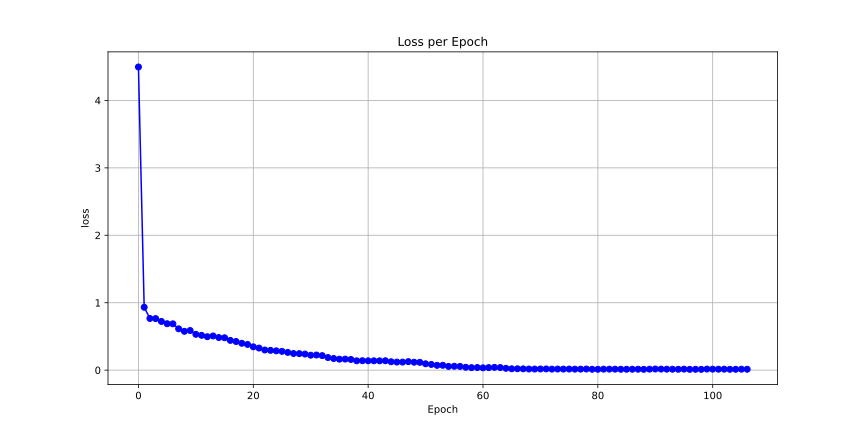
\includegraphics[width=1.3\textwidth, height=1.3\textheight, keepaspectratio]{img/LossPerEpoch.png}}
    \caption{Loss per epoch graph.}
\end{figure}
\subsection{Precision per epoch}
\begin{figure}[H]
    \centering
    \makebox[\textwidth][c]{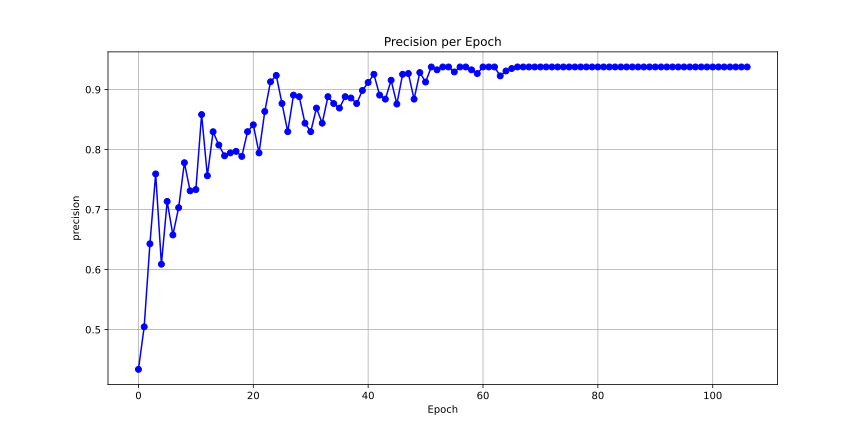
\includegraphics[width=1.2\textwidth, height=1.2\textheight, keepaspectratio]{img/PrecisionPerEpoch.png}}
    \caption{Precision per epoch graph.}
\end{figure}
\subsection{Recall per epoch}
\begin{figure}[H]
    \centering
    \makebox[\textwidth][c]{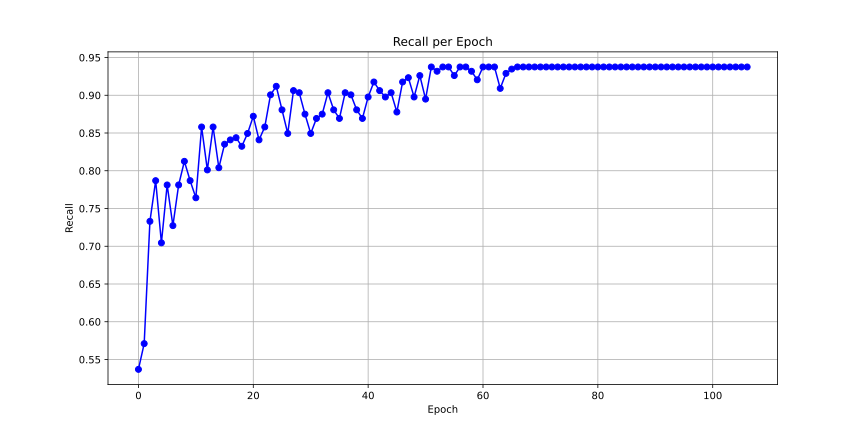
\includegraphics[width=1.2\textwidth, height=1.2\textheight, keepaspectratio]{img/RecallPerEpoch.png}}
    \caption{Recall per epoch graph.}
\end{figure}
\subsection{ROC/AUC per epoch}
\begin{figure}[H]
    \centering
    \makebox[\textwidth][c]{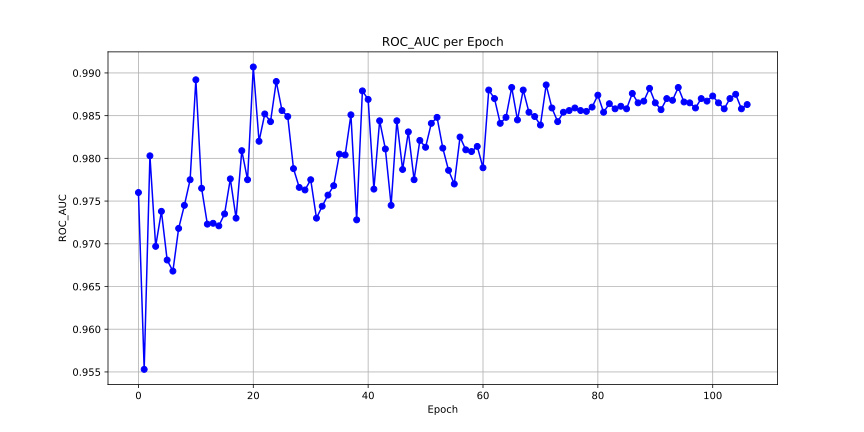
\includegraphics[width=1.2\textwidth, height=1.2\textheight, keepaspectratio]{img/ROC_AUCPerEpoch.png}}
    \caption{ROC/AUC per epoch graph.}
\end{figure}
\subsection{F1score per epoch}
\begin{figure}[H]
    \centering
    \makebox[\textwidth][c]{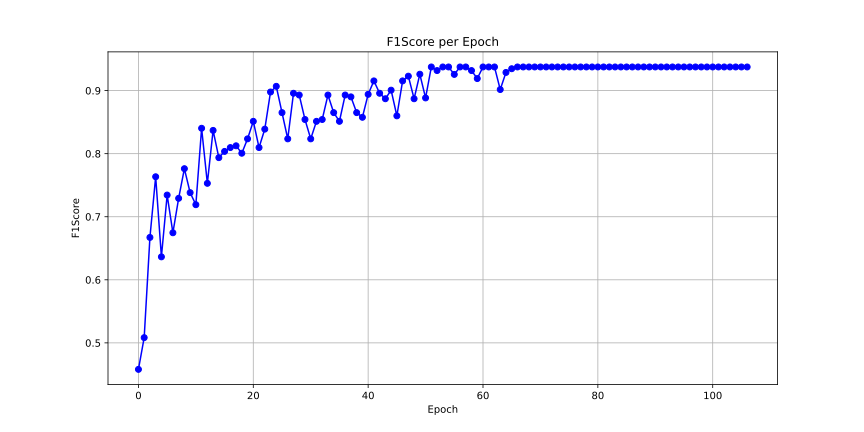
\includegraphics[width=1.2\textwidth, height=1.2\textheight, keepaspectratio]{img/F1ScorePerEpoch.png}}
    \caption{F1score per epoch graph.}
\end{figure}
\subsection{ROC}
\begin{figure}[H]
    \centering
    \makebox[\textwidth][c]{\includegraphics[width=0.7\textwidth, height=0.7\textheight, keepaspectratio]{img/ROC curve.png}}
    \caption{ROC graph.}
\end{figure}
\subsection{Confusion matrix}
\begin{figure}[H]
    \centering
    \makebox[\textwidth][c]{\includegraphics[width=0.7\textwidth, height=0.7\textheight, keepaspectratio]{img/Confusion Matrix.png}}
    \caption{Confusion matrix.}
\end{figure}
\subsection{Results analysis}
\begin{itemize}
    \item Loss per epoch graph: The graph shows that the loss consistently decreases as the training progresses, indicating that the model is learning and improving its predictions. Once the loss reaches a certain threshold, it begins to stabilize, suggesting that the model has converged and further improvements may be minimal.
    \item Precision per epoch graph: As training progresses, the precision of the model gradually improves, indicating that it's getting better at correctly identifying true positives while reducing false positives. This means the model is becoming more selective and making fewer incorrect positive predictions. Once precision reaches a certain threshold, it stabilizes, suggesting that the model has fine-tuned its ability to focus on the most relevant predictions without further unnecessary improvements.
    \item Recall per epoch graph: Similarly, recall increases over time, showing that the model is effectively capturing more true positives and reducing false negatives. This reflects the model's growing ability to identify relevant instances in the dataset. Once recall hits a certain level, it stabilizes, indicating that the model has reached a consistent level of sensitivity in finding positive cases, with little room for further enhancement.
    \item ROC/AUC per epoch graph: This graph shows how the ROC AUC score changes over epochs during training. Initially, the AUC shows fluctuations, indicating variability in model performance as it learns. Over time, the AUC stabilizes around a high value, suggesting that the model is converging and maintaining strong discriminatory ability between classes.
    \item F1score per epoch graph: The F1 score, which balances precision and recall, shows an upward trend with initial fluctuations, reflecting the model's improving ability to balance false positives and false negatives. Eventually, the score stabilizes, indicating that the model reaches consistent performance in classification tasks.
    \item ROC graph: The graph shows that the ROC curve almost perfectly follows the left-hand border and then the top border, indicating excellent classification performance.
    \item Confusion matrix: The diagonal cells represent the correctly classified instances, which are mostly concentrated with high values, indicating that the model performs well across most classes. The off-diagonal cells represent the misclassifications, which appear to be minimal, further reinforcing the model's effectiveness. The model almost perfectly classifies except for class 1 and 2.
\end{itemize}
\chapter{Conclusion}
In conclusion, this project successfully achieved its objectives by building and optimizing a Convolutional Neural Network (CNN) for image classification. Through various experiments, including adjustments to model architecture, hyperparameters, and preprocessing techniques, the model's performance was significantly improved. The use of Explainable AI techniques provided valuable insights into the model's behavior, enhancing the understanding of how it makes predictions. The implementation of the application demonstrated the practical application of the model, enabling real-time classification on devices. Overall, the project contributes to the field of image classification by combining model optimization with real-world deployment and explainability.
\bibliography{MyBib}

\end{document}
